
The choice of the level of the comparator threshold plays a very important role in counting systems since it influences the efficiency of the detector as well as its spatial resolution (for details see the paper Bergamaschi, A. et al. (2010). J. Synchrotron Rad. 17, 653-668).


Single-photon-counting detectors are sensitive to single photons and the only limitation on the fluctuations of the number of counts is given by the Poisson-like statistics of the X-ray quanta. 
The digitized signal does not carry any information concerning the energy of the X-rays and all photons with an energy larger than the threshold are counted as one bit. This means that the choice of the correct comparator threshold level is critical in order to obtain good-quality data.\\
 Figure~\ref{fig:thrscanexpl} shows the expected number of counts as a function of the threshold energy for $N_0$ monochromatic X-rays of energy $E_0$. This is often denominated  S-curve and can be interpreted as the integral of the signal spectrum between the threshold level and infinity.
The dashed curve represents the behavior of an ideal counting system: nothing is counted for thresholds larger than the photon energy and all the $N_0$ X-rays are counted for thresholds lower than $E_0$.
The thick solid line represents the physical curve which also takes into account the electronic noise and the charge sharing between channels.

The intrinsic noise on the electronic signal  is defined by the Equivalent Noise Charge ($ENC$). The $ENC$ describes noise in terms of the charge at the detector input needed to create the same output at the end of the analog chain and is normally expressed in electrons. For silicon sensors, it can be converted into energy units by considering 1~$e^-$=3.6~eV.
The value of the $ENC$ normally depends on the shaping settings of the analog chain and increases with shorter shaping times. 
The resulting electronic signal spectrum is then  given by a convolution between the radiation spectrum and the noise i.e., a Gaussian of standard deviation $ENC$.  
The S-curve for a monochromatic radiation beam is well described by a Gaussian cumulative distribution $D$ with an additional increase at low threshold due to the baseline noise, as shown by the solid thin line. 

Moreover, when a photon is absorbed in the region between two strips of the sensor, the generated charge is partially collected by the two nearest electronic channels. For this reason the physical S-curve is not flat but can be modeled by a decreasing straight line. The number of shared photons  $N_S$ is given by the difference between the number of counts and the number of X-rays whose charge is completely collected by the strip (shown by the dotted line).

The number of counts in the physical case is equal to that in the ideal case for a threshold set at half the photon energy. This defines the optimal threshold level $E_t=E_0/2$.\\
The detector response $N$ as a function of the threshold energy $E_t$ is given by the sum of the noise counts  $N_n$ and the counts originating from photons $N_\gamma$:
\begin{equation}
N_\gamma(E_t)=\frac{N_0}{2}\cdot\Big(1+C_s \frac{E_0-2E_t}{E_0}\Big)D \Big(\frac{E_0-E_t}{ENC} \Big), \label{eq:thrscan}
\end{equation}
where $C_s$ is the fraction of photons which produce a charge cloud which is shared between neighboring strips ($N_s=C_s N_0$).\\
By assuming a noise of Gaussian type, and considering its bandwidth limited by the shaping time  $\tau_s$, the number of noise counts in the acquisition time $T$ can be approximated as:
\begin{equation}
N_n(E_t) \sim \frac{T}{\tau_s}  D \Big(\frac{-E_t}{ENC} \Big). \label{eq:noisescan}
\end{equation} 

The choice of the comparator threshold level $E_t$ influences not only the counting efficiency and noise performances, but also the spatial resolution and the counting statistics of the detector. 
If the threshold is set at values higher than the ideal value $E_t=E_0/2$, a fraction of the photons absorbed in the sensor in the region between two strips is not counted thus reducing the detector efficiency but improving its spatial resolution (narrower strip size). On the other hand, if the threshold is set at values lower than $E_t$, part of the X-rays absorbed in the region between two strips are counted by both of them, resulting in a deterioration of the spatial resolution of the detector and of the fluctuations on the number of photons because of the increased multiplicity. 


Furthermore, the threshold uniformity is particularly critical with regards to fluorescent radiation emitted by the sample under investigation. Since the emission of fluorescent light is isotropic, the data quality will be improved by setting the threshold high enough in order to discard the fluorescence background (see figure~\ref{fig:thrscanfluo}). \\
Moreover, setting the threshold too close to the energy of the fluorescent light gives rise to large fluctuations between channels in the number of counts since the threshold sits on the steepest part of the threshold scan curve for the fluorescent background. These differences cannot be corrected by using a flat-field normalization  since the fluorescent component is not present in the reference image. For this reason, it is extremely important that the threshold uniformity over the whole detector is optimized. The threshold level must be set at least $\Sigma>3\,ENC$ away from both the fluorescent energy level and the X-ray energy in order to remove the fluorescence background while efficiently count the diffracted photons. 

The comparator threshold is given by a global level which can be set on a module basis and adds to a component which is individually adjustable for each channel. In order to optimize the uniformity of the detector response it is important to properly adjust the threshold for all channels. \\
Since both the signal amplification stages and the comparator  are linear, it is necessary to calibrate the detector offset $O$ and gain $G$ in order to correctly set its comparator threshold $V_t$ at the desired energy $E_t$:
\begin{equation}
V_{t}=O+G \cdot E_t.\label{eq:encal}
\end{equation}
This is initially performed by acquiring measurements while scanning the global threshold using different X-ray energies and calculating the median of the counts at each threshold value for each module $i$. The curves obtained for one of the detector modules at three energies are shown in figure~\ref{fig:modulecalibration}. The experimental data are then fitted according to equation~\ref{eq:thrscan} and for each module a linear relation is found between the X-ray energy and the estimated inflection point, as shown in the inset of figure~\ref{fig:modulecalibration}. The resulting offset  $O_i$ and  gain $G_i$ are used as a conversion factor between the threshold level and the energy. 


\begin{figure}
\caption{Expected counts as a function of a threshold energy for a monochromatic beam of energy $E_0$=12~keV. $N_0$=10000 is the number of photons absorbed by the detector during the acquisition time. The dashed line represents the curve in an ideal case without electronic noise and charge sharing, the solid thin line with noise  $ENC$=1~keV but without charge sharing and the solid thick line is the physical case with noise and $CS=$22~\% charge sharing. $N_S$ is the number of photons whose charge is shared between neighbouring strips ($CS=\frac{N_S}{N_0}$). The dotted line represents the number of photons whose charge is completely collected by a single strip.}\label{fig:thrscanexpl}
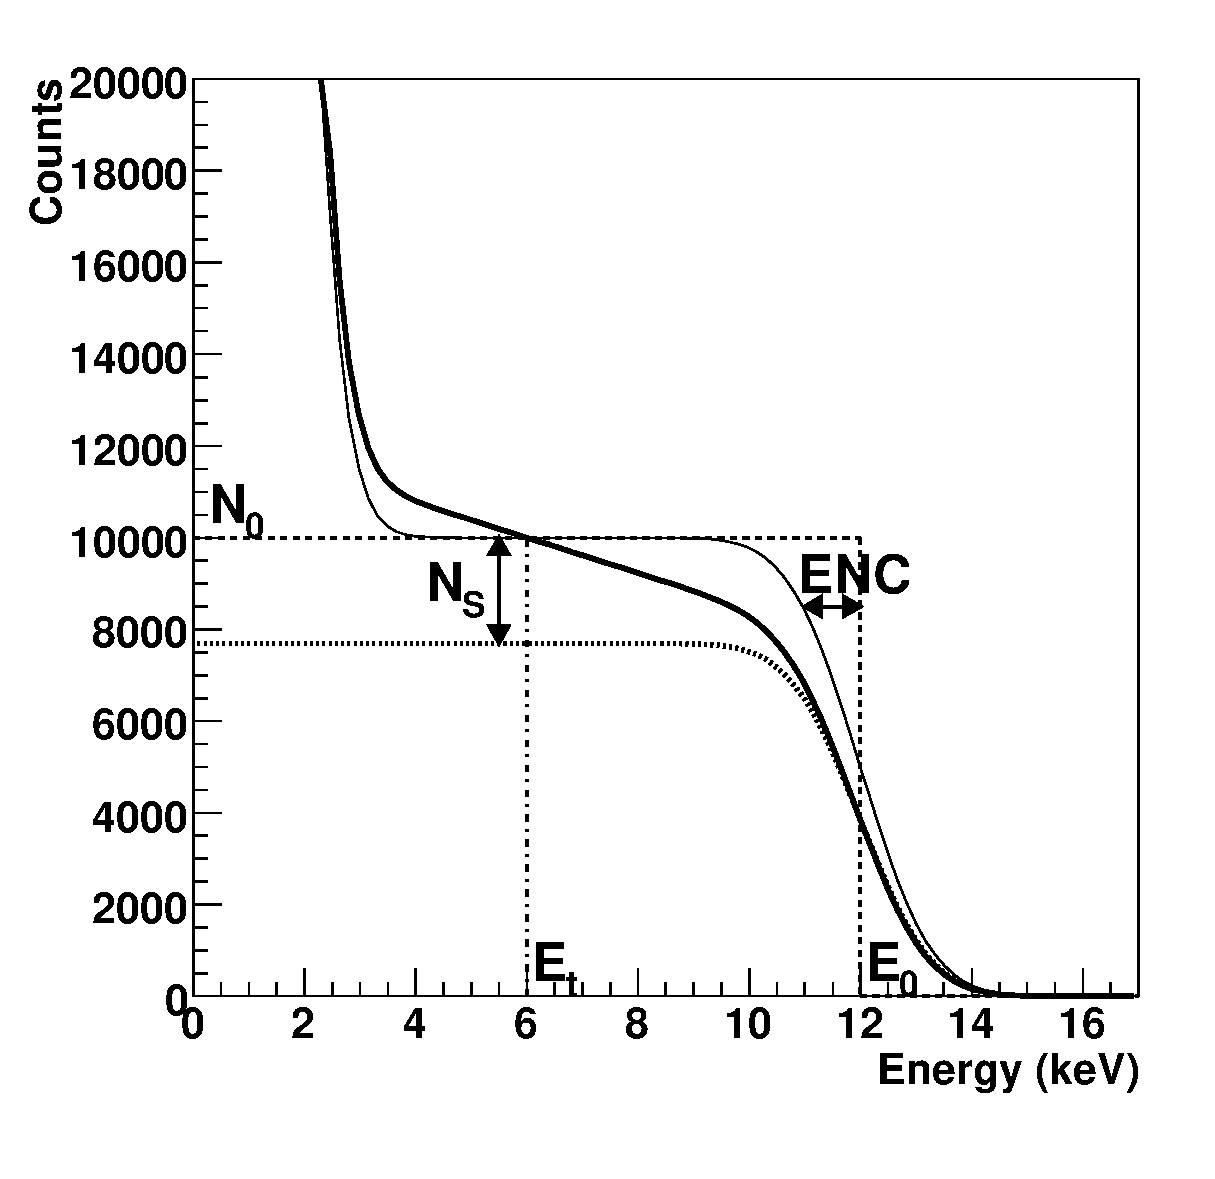
\includegraphics[width=\textwidth]{fig4.eps}
\end{figure} 



\begin{figure}
\caption{Measured threshold scan at 12.5~keV with the three different settings. In the inset the fit of the experimental data with the expected curve as in function~\ref{eq:thrscan} is shown in the region of the inflection point.} \label{fig:expthrscan}
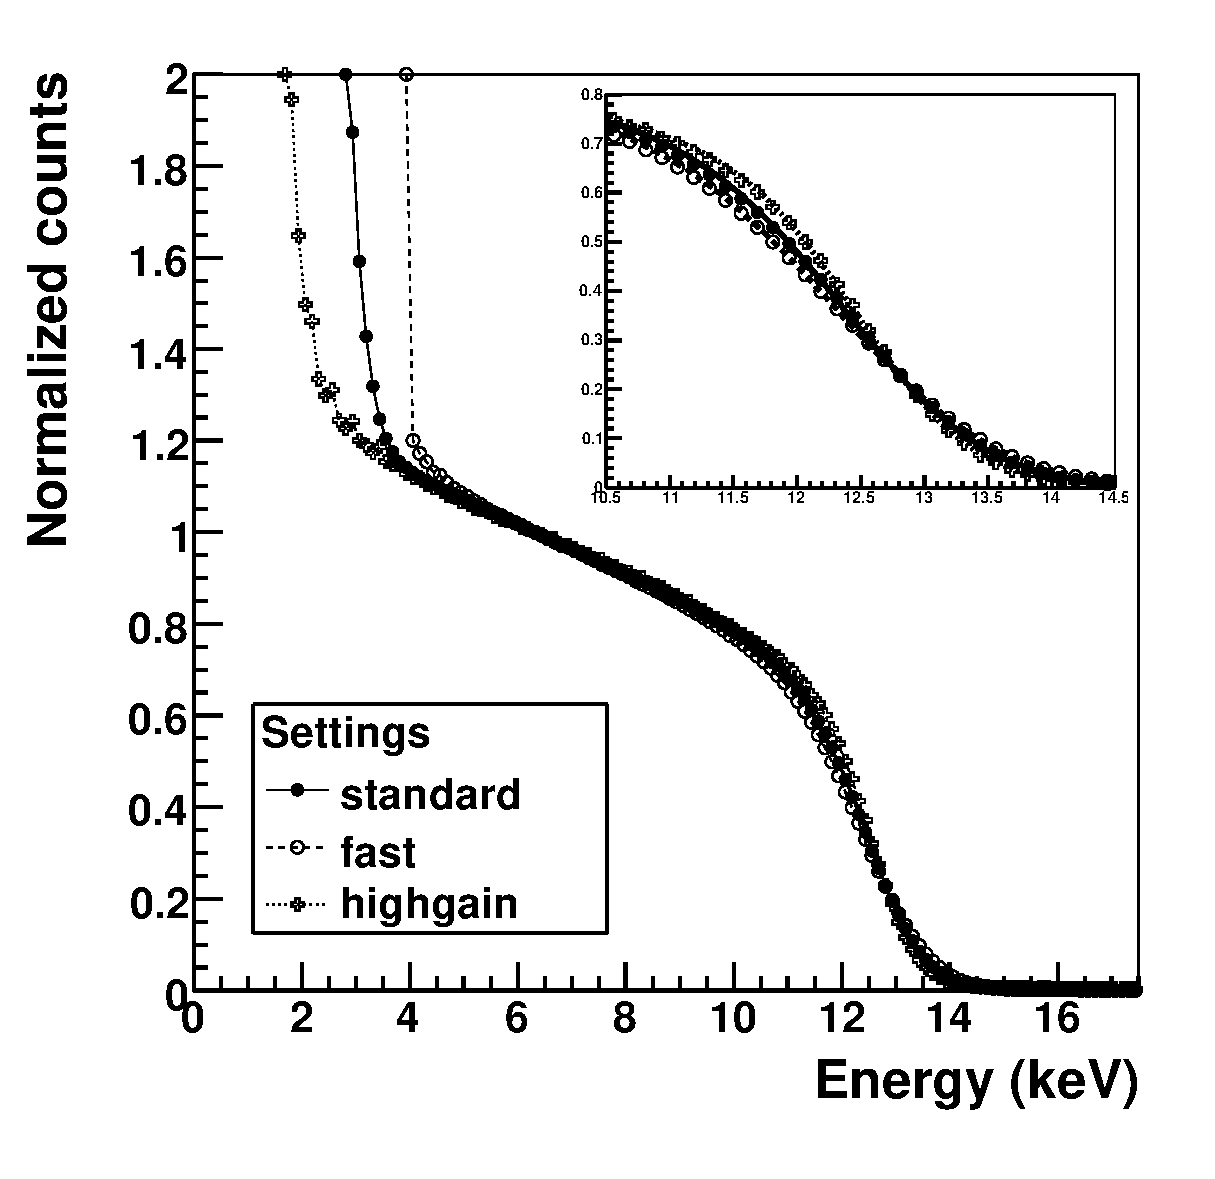
\includegraphics[width=\textwidth]{fig5.eps}
\end{figure} 

\begin{figure}
\caption{Number of counts as a function of the threshold measured from a sample containing iron ($E_f$=5.9~keV) when using X-rays of energy $E_0$=12~keV. In this case, setting the threshold at $E_0/2$, which is very close to $E_f$, would give $\Delta \sim$10\% counts from the fluorescense background. Therefore the threshold should be set at an intermediate level $E_t$ between the two energy components with a distance of at least $\Sigma>3ENC$  from both $E_f$ and $E_0$.}\label{fig:thrscanfluo}
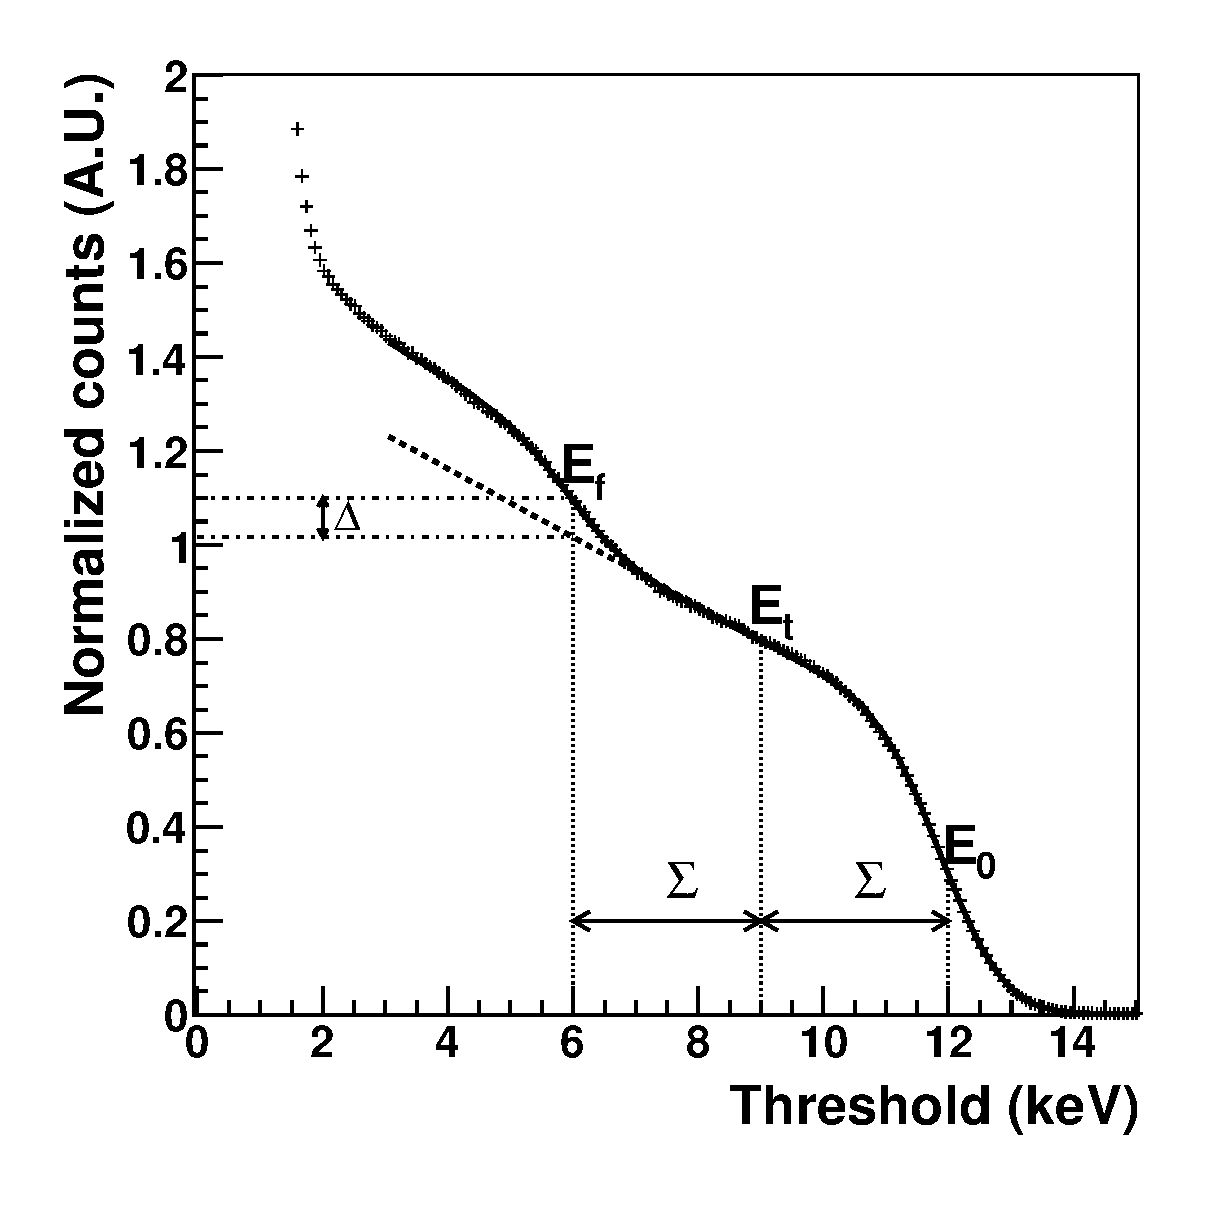
\includegraphics[width=\textwidth]{fig7.eps}
\end{figure}
Differences in gain and offset are present also between individual channels within a module and therefore the use of threshold equalization techniques (trimming) using the internal 6-bit DAC is needed in order to reduce the threshold dispersion.
Since both gain and offset have variations between channels, the optimal trimming should be performed as a function of the threshold energy.
Please not that trimming of the channels of the detector should be performed in advanced and is extremely important for a succeful energy calibration of the detector.

All energy calibration procedures should be applied to a trimmed detector and only an improvement of the existing trimbits can be performed afterwards, since it does not significatively affect the energy calibration.


\begin{figure}
\caption{Median of the number of counts as a function of the threshold for X-rays of 12.5, 17.5 and 25~keV for one of the detector modules using \textit{standard} settings. The solid line represents the fit of the experimental points with equation~\ref{eq:thrscan}. In the inset the linear fit between the X-ray energy and the position of the inflection point of the curves is shown.}\label{fig:modulecalibration}
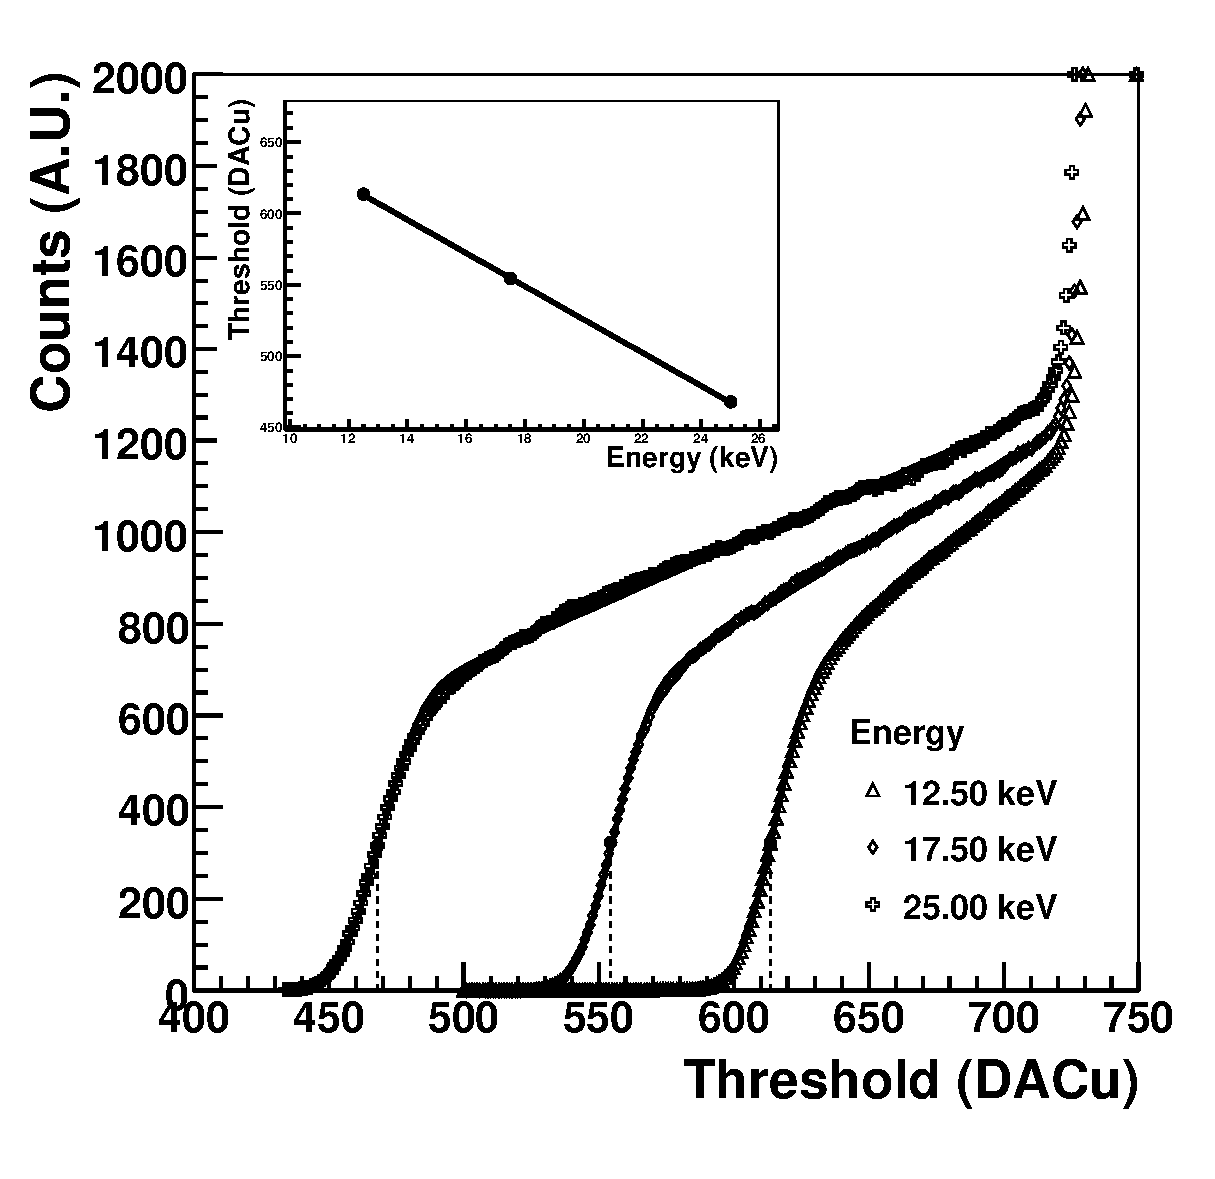
\includegraphics[width=\textwidth]{fig8.eps}
\end{figure}
\newpage

\section{Data acquisition}

The energy calibration consists in acquiring threshold scans using the detector at at least 2 (better 3) energies. A monochromatic beam is ideal in this procedure, but beam obtained from some fluorescent sample is also good.\\
Please note that the statistic is important to succesfully analyze the data. Normally the exposure time for each step should be chosen in order to achieve at least 1000 counts per step.
If this is not possible it is better to reduce the scan range or enlarge the scan step rather than acquiring data with a too low statics.

With a quick acquisition or threshold scan it is useful to define the range of the scan and the exposure time. It is important to start from a threshold high enough that (almost) all channels of the detector have a negligible number of counts and that the plateau of the S-curve is long enough to correctly estimate the number of photons.

\subsection{Software}

For the acquisition ot the data you need to install the slsDetector software package (please refere to separate documentation). The use of the GUI is optional and all operations can be performed also using the text client.\\

In the following the command to acquire a dataset for the energy calibration with an exposure time of 1~s, and threshold scan range between 200 and 850 with a setp of 1 DAC unit.
\begin{verbatim}
> sls_detector_put encallog 1 #setup energy calibration
> sls_detector_put exptime 1. #set exposure time to 1s
> sls_detector_put scan0script threshold #setup threshold scan
> sls_detector_put scan0range 200 850 1 #set scan range between 200 and 850, step of 1
> sls_detector_acquire #acquire the data
> sls_detector_put encallog 0 #unset energy calibration
\end{verbatim}

With the GUI you can obtain the same results by clicking on the \textit{Energy Calibration} log button in the advanced tab (see figure~\ref{fig:guiencallog}) and setting up the threshold scan in the Actions tab (see figure~\ref{fig:guithrscan}). the exposure time should also be set in the measurement tab.


This procedure should be executed at at least 2 (better 3) energies.

Additional to the data files, the acquisition will produce a .encal file containing an header and, for each step of the acquisition, the threshold value and the file name. \\
In case you forgot to enable the encallog flag in the software, you can produce the file with the syntax as follows:
\begin{verbatim}
settings standard
type Mythen+
nmod 12
modulenumber:0 000
modulenumber:1 111
modulenumber:2 222
modulenumber:3 333
modulenumber:4 444
modulenumber:5 555
modulenumber:6 666
modulenumber:7 777
modulenumber:8 888
modulenumber:9 999
modulenumber:10 aaa
modulenumber:11 bbb
450 standard_12_4keV_S450_0
460 standard_12_4keV_S460_0
470 standard_12_4keV_S470_0
480 standard_12_4keV_S480_0
490 standard_12_4keV_S490_0
500 standard_12_4keV_S500_0
510 standard_12_4keV_S510_0
520 standard_12_4keV_S520_0
...
...
\end{verbatim}




\begin{figure}
\caption{Acquisition GUI window to enable the energy calibration log.} \label{fig:guiencallog}
\includegraphics[width=\textwidth]{GUI_Advanced.eps}
\end{figure} 

\begin{figure}
\caption{Acquisition GUI window to setup the threshold scan.} \label{fig:guithrscan}
\includegraphics[width=\textwidth]{GUI_ThresholdScan.eps}
\end{figure} 
\newpage

\section{Data analysis}

The data analysis consists in fitting the S-curves obtained from the datasets acquired as above and then performing a linear fit between the energy values and the inflection points.

\subsection{Software}

The software used for the energy calibration data analysis is based on root (see http://root.cern.ch).\\
This can be downloaded as binary or installed from sources. The version of the software should not play an important role, but up to now everything has been implemented and tested using version 5.20.

To start the data analysis simply launch:
\begin{verbatim}
> ./energyCalibrationWizard 
\end{verbatim}

To add anew energy write the energy value and select (or digit) the name of the .encal file corresponding to that energy (see figure~\ref{fig:addenergy}).\\
The software assumes that the data files (.raw) and the .encal file are in the same directory.
Press  \textit{Preview} and a 2D color plot will be displayed, showing the channel numbers on the X-axis, the threshold on the Y-axis, and the number of counts as a color scale.
By (right) clicking close to the axis you are able to zoom in/out, set the scale to logarithmic etc.\\
If the plot corresponds to your expectations press \textit{Add to list}. The energy value will be shown in the combo box on top and labels will display the settings of the detector, the number of modules, the number of channels per module and the modules serial numbers.

Add then all the other energies to the calibration always by editing the energy value and .encal file name, pressing \textit{preview} and \textit{add to list}.\\
If the settings, number of modules or serial numbers do not match, you will not be llowed to add the energy.\\
By using the \textit{selected energy actions} you can navigate in the combo box with list of energies, view the plots and eventually remove the ones you don't want to use in your calibration.\\
Once you have uploaded at least 2 energies, you will be allowed to  \textit{proceed to module calibration}.



\begin{figure}
\caption{Window to add energies to the calibration.} \label{fig:addenergy}
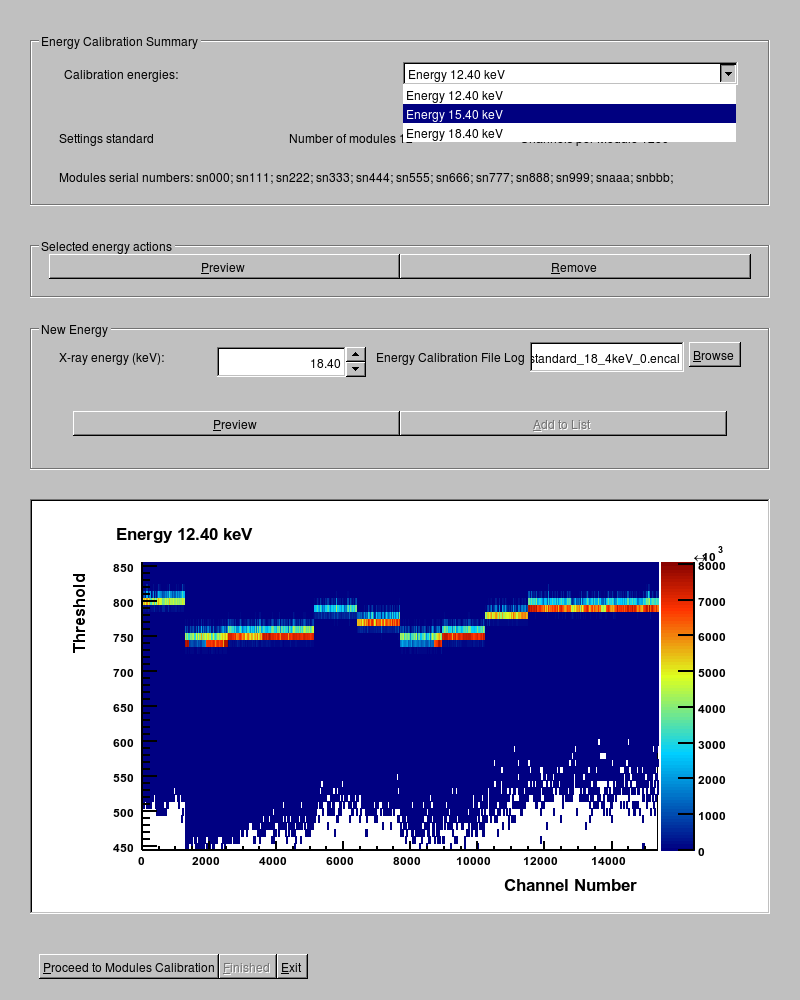
\includegraphics[width=\textwidth]{addEnergy.eps}
\end{figure} 

In the module calibration window (see figure~\ref{fig:calibratemodule}), you are still able to look at the calibration summary, and eventually return to the previous windown by pressing \textit{Back to energy setup}.\\
The canvas will show the plot of the S-curves relative to the median of the selected module, fitted with equation~\ref{eq:thrscan} and the linear fit between the energy values and the fitted inflection points.
Normally the points lie on a straight line (although often not perfect), therefore it should be simple to spot if there are problems in the fitting of some of the data.\\
If \textit{Manual save} is unclicked, the calibration files will be saved locally, with the extension automatically generated by using the modules serial numbers, every time a linear fit is performed (i.e. if you mess up wiht the linear fit you overwrite a previous good file!). If you click the checkbox, you need to save the calibration by pressing \textit{Write to file} for each module once you are happy with the fit.

To change the Y scale of the plot, edit the \textit{Counts} entry. After clicking of the energy button (eventually twice) the maximum of the histogram will be set to three times the value.

To re-fit one energy with modified range or start parameters, you should press the central button with the energy value once the energy is selected. The text color tells you which curve you are referring to.\\

You should set the range of the fit. In particular the maximum should be limited in order to avoid to enter the noise range (and can be pretty different for the various modules).\\
Normally the data are acquired by collecting holes from the detector and therefore the \textit{Invert axis} check button should be ckecked. Uncheck it in case your detector collects electrons (e.g. CdTe, Si n in p)

You can change the start values of the parameters of the fits by editing the number eneries. The label nearby will show you the actual value of the fitted parameters.\\
By checking the checkboxes you can fix the values to the ones you specify.\\
Normally it can be useful to fix the pedestal and pedestal slope to 0, unless you have a lot of 3rd armnonics contribution, primary beam background or similar.\\
Changing the starting value of the inflection point or of the number of counts can often help the fit to converge.\\
Normally it is not very useful to change the starting value for the noise or charge sharing slope.

The button \textit{Finished} will be enebled only once the calibration files have been generated for all modules.


\begin{figure}
\caption{Window to calibrate the modules.} \label{fig:calibratemodule}
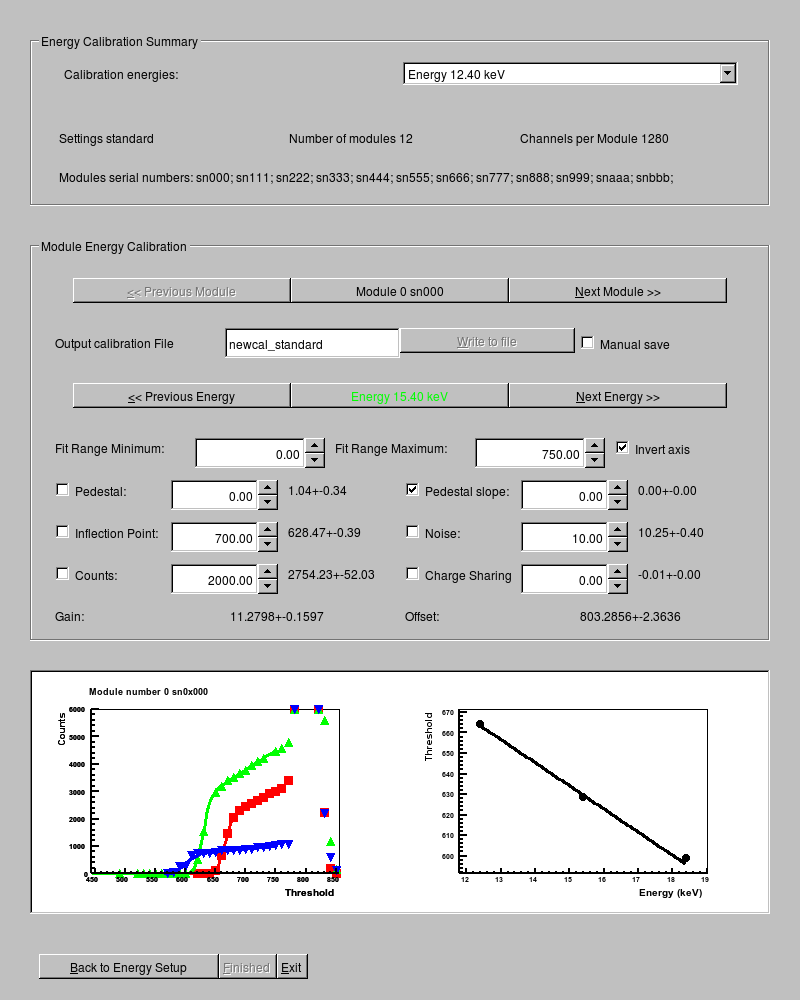
\includegraphics[width=\textwidth]{calibrateModule.eps}
\end{figure} 
\newpage


\section{Setup calibration files}

To use the genrated calibration files as default ones, copy them into your default \textit{caldir/settings} renaming them calibration.snxxx, where snxxx is the extension that the genrated files already have, which corresponds to the module serial number.\\
Fot this scope, a script as following can be used:
\begin{verbatim}
for i in $(ls newcal_standard.sn* | awk -F "." '{print $2}'); do \
mv newcal_standard.$i caldir/standard/calibration.$i; \
done
\end{verbatim}

By reloading the default detector settings, the calibration coefficients will be automatically loaded.
